\documentclass[12pt]{article}
\usepackage{graphicx}
\usepackage{amssymb}
\usepackage{epstopdf}
\usepackage{amsmath}
\usepackage{multicol}
\usepackage{tcolorbox}
\usepackage{geometry}
\usepackage{enumitem}
\usepackage{fancyhdr}

\DeclareGraphicsRule{.tif}{png}{.png}{`convert #1 `dirname #1`/`basename #1 .tif`.png}

\textwidth = 6.5 in
\textheight = 9 in
\oddsidemargin = 0.0 in
\evensidemargin = 0.0 in
\topmargin = -23pt
\headheight = 0.0 in
\headsep = 0.0 in
\parskip = 0.2in
\parindent = 0.0in
\pagestyle{fancy}
\pagenumbering{gobble}

\newtheorem{theorem}{Theorem}
\newtheorem{corollary}[theorem]{Corollary}
\newtheorem{definition}{Definition}
%\includegraphics [height=50mm, width=50mm]{PathInt.jpg}
\title{Title} 

\begin{document}
%INSTRUCTOR NOTES
%No warm-up on quiz days. If wanted, today's warm-up would be solving equations.
 Name:
 \begin{center}\large{3.2.0 Exponent and Log Review}\end{center}


\begin{tcolorbox}

\textbf{Properties of Exponents:}
\begin{multicols}{3}
	\begin{enumerate}[itemsep=.6cm]
	\item $\displaystyle a^na^m= $\underline{\hspace{2cm}} 
	\item $\displaystyle \frac{a^n}{a^m}= $\underline{\hspace{2cm}} 
	\item $\displaystyle (a^n)^m= $\underline{\hspace{2cm}} 
	\item $\displaystyle (ab)^n= $\underline{\hspace{2cm}} 
	\item $\displaystyle \left(\frac{a}{b}\right)^n= $\underline{\hspace{2cm}} 
\item $\displaystyle a^0= $\underline{\hspace{2cm}} 
\item $\displaystyle a^{-n}= $\underline{\hspace{2cm}} 
\item $\displaystyle a^{\frac{1}{n}}= $\underline{\hspace{2cm}} 
\item $\displaystyle a^{\frac{m}{n}}= $\underline{\hspace{2cm}} 
\end{enumerate}
\end{multicols}

\textbf{Logarithms:} \\
If $\log_{a} x = y$, ...\\




\textbf{Facts about Logarithms:} 


\begin{multicols}{3}
	\begin{enumerate}[itemsep=.6cm]


\item $\log x$ is ...
\item $\ln x$ is ...

\item $\log_{a}(a^x)=$

\item $a^{\log_{a}x}=$


\item $\log_a(nm)=$

\item $\log_a(\frac{n}{m})=$

\item  $\log_a(n^t)=$

\item $\log_a 1=$

\item $\log_a a=$

\end{enumerate}
\end{multicols}
\end{tcolorbox}

\begin{enumerate}
\item Simplify the following expressions. 
	\begin{multicols}{2}
	\begin{enumerate}[itemsep=2cm]
	\item $\displaystyle \left(\frac{5a^{0}b^{3}}{a^{3}b^{-2}}\right)^{-2}$
	
	\item $\displaystyle \ln\left(e^{2}\right)$
	
	\item $\displaystyle \log_{2}\left(\frac{1}{8}\right)$
	
	\item $\displaystyle \sqrt{t}(t^2-3t+2)$
	
	\item $\displaystyle \frac{x^3y^{-1}+x}{\sqrt{x^3}}$
	
	\item $\displaystyle 2c^{-1}(c^2+c)-2$
	\end{enumerate}
	\end{multicols}
\newpage

~
\item Solve the following equations for $x$.
	\begin{multicols}{2}
	\begin{enumerate}[itemsep=4cm]
	\item $\displaystyle \log\left(3x^{3}\right)=2$
	
	\item $\displaystyle 15e^{\left(3x+5\right)}=5$
	
	\item $\displaystyle 7\cdot2^{x}=2\cdot3^{x}$
	
	\item $\displaystyle 25x^{5}=100$
	\end{enumerate}
	\end{multicols}
\vfill
\item Match the graph on the left to the function equation on the right. (Yes, multiple equations match the same graph.)\\
\noindent\begin{minipage}{0.7\textwidth}% adapt widths of minipages to your needs
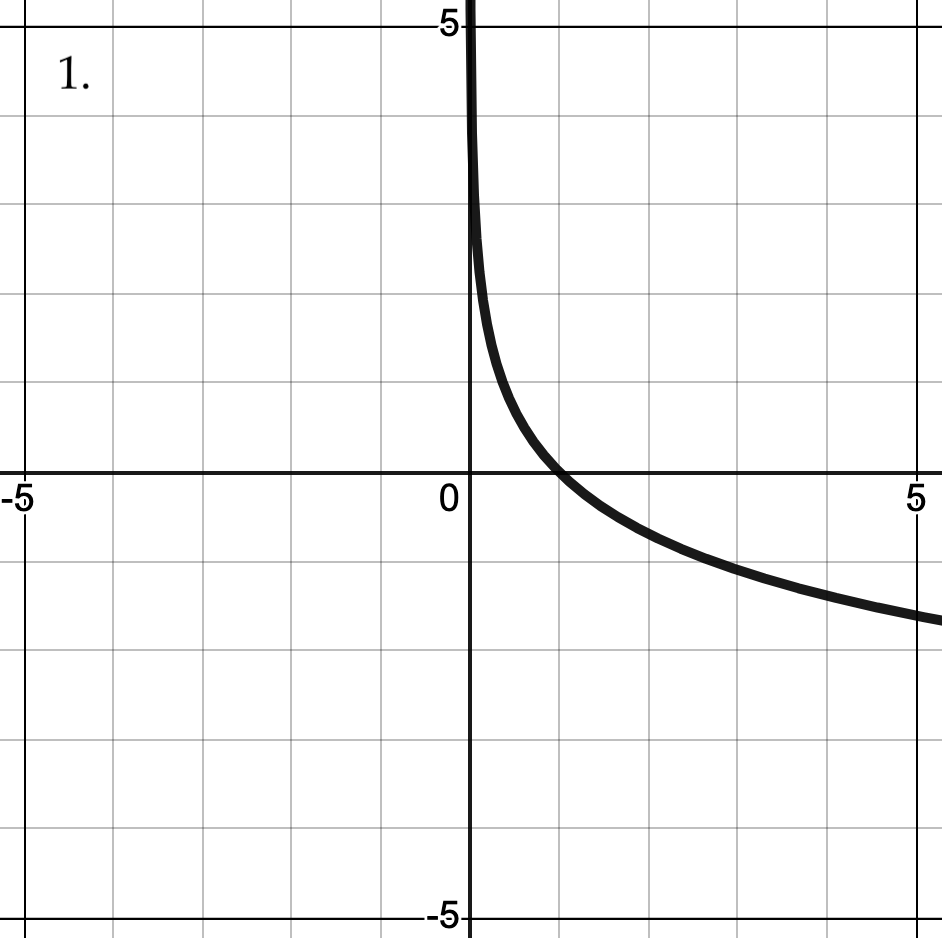
\includegraphics [scale=.15]{3_2_0_gd}
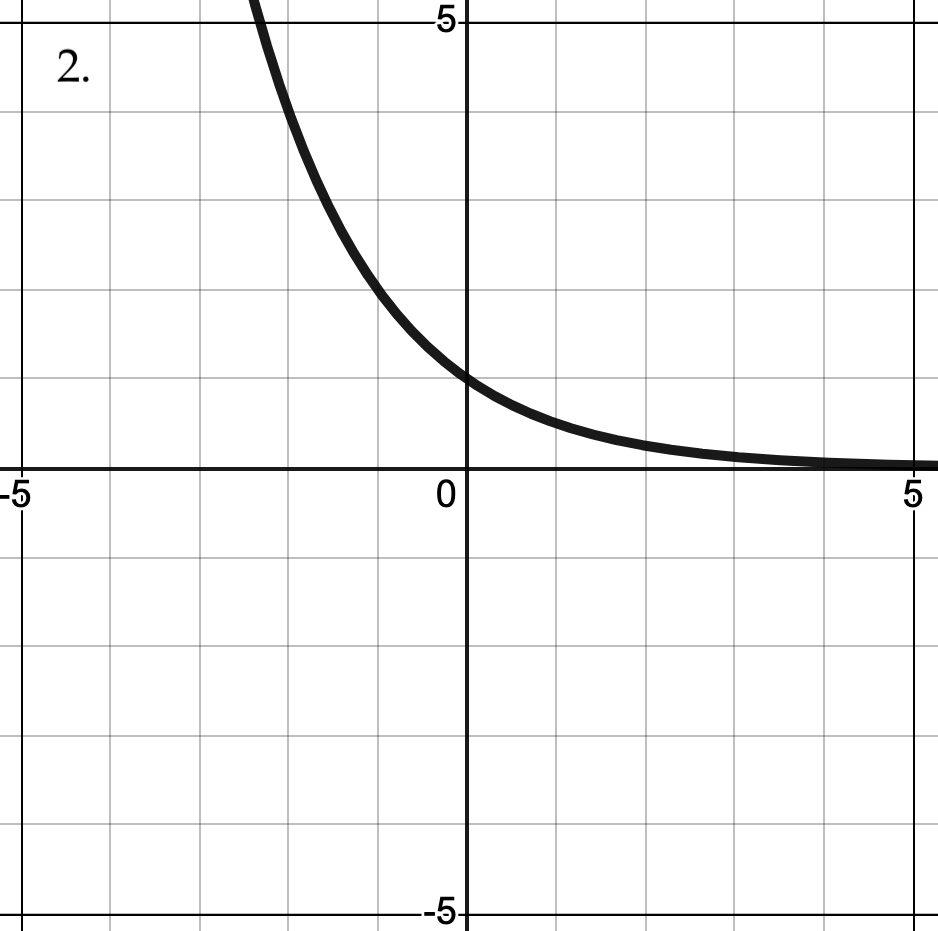
\includegraphics [scale=.15]{3_2_0_gb}\\
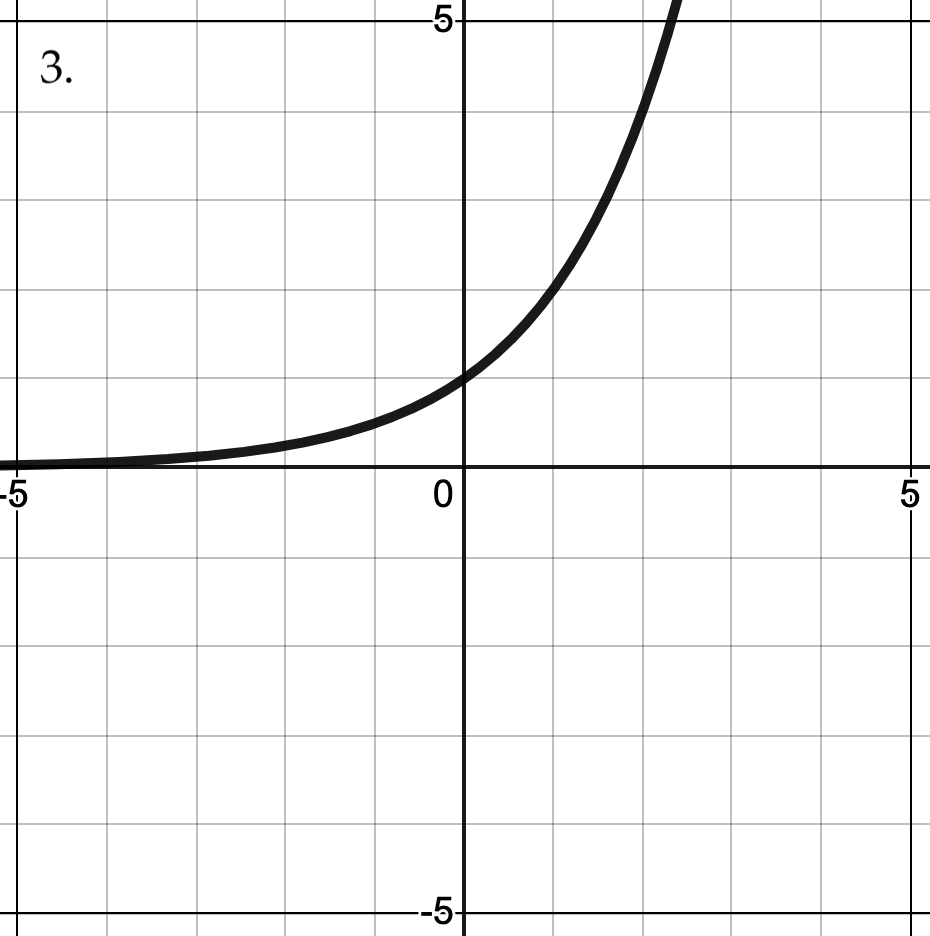
\includegraphics [scale=.15]{3_2_0_ga}
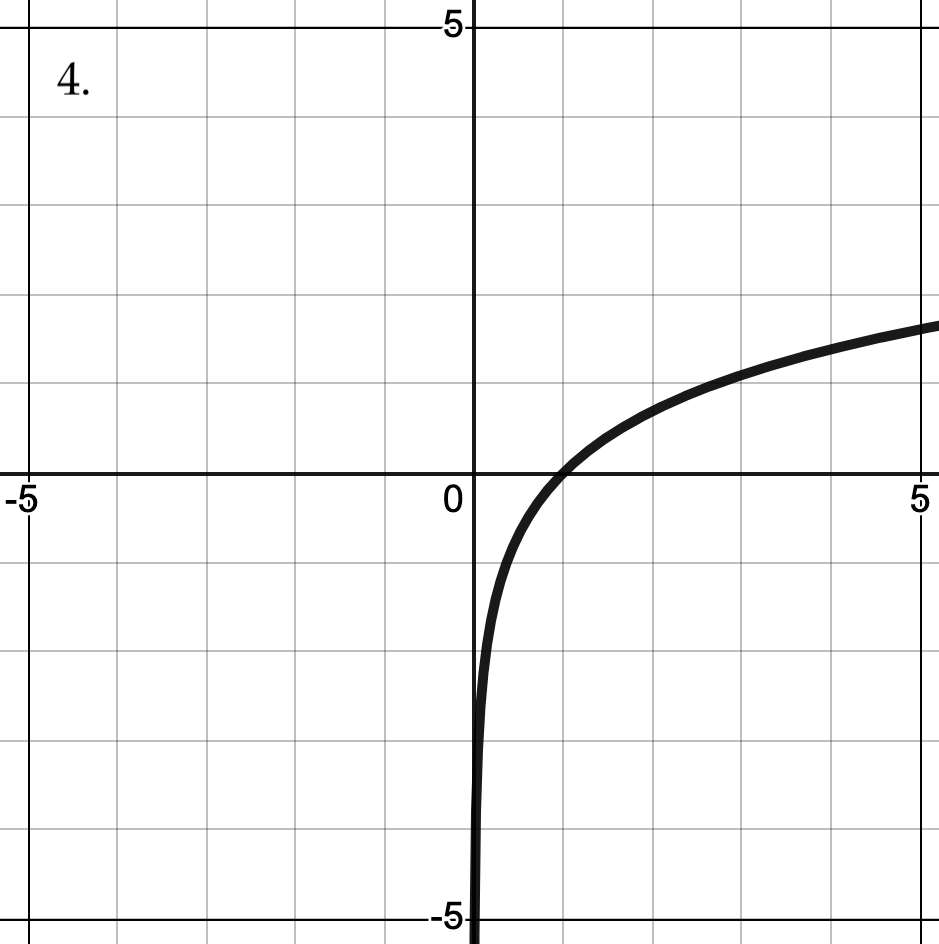
\includegraphics [scale=.15]{3_2_0_gc}
\end{minipage}%
\hspace{5mm}
\begin{minipage}{0.6\textwidth}

a) $f(x)=2^x$\\

\vspace{10mm}
b) $g(x)=2^{-x}$\\

\vspace{10mm}
c) $\displaystyle h(x)=\left(\frac{1}{2}\right)^x$\\

\vspace{10mm}
d) $k(x)=\ln(x)$\\

\vspace{10mm}
e) $m(x)=-\ln(x)$
\end{minipage}


	

	
\end{enumerate}
\end{document} 

%%%%%%%%%
\begin{tcolorbox}
\textbf{Warm-up: } Solve the following equations for $t$.
\begin{multicols}{2}
\begin{enumerate}
\item $(t+1)^2=9$
\item $tx+x^2=5$
\end{enumerate}
\end{multicols}
\end{tcolorbox}

MINIPAGE
\noindent\begin{minipage}{0.3\textwidth}% adapt widths of minipages to your needs
try 1
\end{minipage}%
\hspace{40mm}
\begin{minipage}{0.6\textwidth}
a) $f'(2)=$\\\

b) $f'(4)=$\\

c) $f'(6)=$\\

d) $f'(7)=$\\

e) $f'(8)=$
\end{minipage}
